\documentclass{thomasClass}

\usepackage{fancyvrb}
\usepackage{fvextra}
\renewcommand{\abstractname}{Introduction}

\setcounter{tocdepth}{1}

\title{\noindent \rule{\textwidth}{1pt}\\ [1cm]
    \textbf{\huge Web Development Languages}\\ For A-Level Computer Science}
\author{Thomas Boxall}
\date{February 2021 (Reviewed in April 2022)\\ [1cm]
    \noindent \rule{\textwidth}{1pt}}

\begin{document}

\maketitle

\begin{abstract}
    This was originally produced as part of a directed study week in 2021. During revision for A-Levels in 2022, this document has been reviewed with additional notes added. At this time, it was also typeset into \LaTeX.\\
    In the examples used in this document, \verb|...| indicates where other code would be inserted.
\end{abstract}

\tableofcontents



\chapter{HyperText Markup Language}
This is the standard markup language used to develop web pages. It comprises of elements which have a \verb|<startTag>| and a \verb|</endTag>|. Some elements do not have end tags, for example, the \verb|<br>| tag. These are known as empty elements.

\section{Elements}
Elements are the building blocks of a HTML document. It is through different elements that a web page is designed and built.
\subsection{Definition of a HTML document}
The \verb|<!DOCTYPT html>| tag must appear at the top of every HTML document. It tells the web browser that the document is a HTML document so that it knows how to output it correctly. The element should appear only once, at the top of every HTML file in the website.
\subsection{Root HTML Element}
\begin{verbatim}
<html>
...
</html>
\end{verbatim}
These tags are used to encapsulate the HTML code which is used to build the web page.
\subsection{Headings}
There are 6 heading tags, the text gets smaller as the number in the tag gets bigger.\\
\verb|<h1> <h2> <h3> <h4> <h5> <h6>|\\
These are used in a pair, a start tag and end tag.\\
\verb|<h1>...</h1>|\\
Browsers will automatically add some white space before and after the heading. Search engines use heading tags to build indexes of what is on pages, this is used in their page rank algorithms. For this reason, do not use heading tags to make text big or bold unnecessary.
\subsection{Paragraphs}
The \verb|<p>| tag is used to define normal text. It is used in the same way as most other tags \verb|<p>...</p>|. A paragraph will always start on a new line and browsers will automatically add some white space before and after the text. The browser will also strip any extra spaces from before and in between the text.
\subsection{Horizontal Lines}
The \verb|<hr>| tag is used to include a horizontal line. They are often used to define a thematic change in the HTML page and separate the page content. This doesn't need an end tag.
\subsection{Line Break}
The \verb|<br>| tag is used to break the line, it is used within other tags (for example, a \verb|<p>|) and doesn't need an end tag.
\subsection{Hyperlinks}
Hyperlinks are fundamental to websites. They allow pages to be linked to other pages, meaning users can move around the website without needing to know the exact URL of each page. The \verb|href| attribute of the \verb|<a>| tag defines where the link should take the user. More information in the Links section.

\section{Styles}
\label{sec:styles}
The HTML \verb|style| attribute is used to add styles to an element such as colour, size or font. The syntax is as follows: \verb|<tagname style="property:value;"|. The property is a CSS property and the value is a CSS value. 
\subsection{Background Colour}
This defines the background colour of a HTML element. For example, to set the background colour of a \verb|<h1>| element saying "Cheese" to powder blue:\\
\verb|<h1 style=”background-color:powderblue;”>Cheese</h1>|\\
Using this syntax, the background colours can be different for different elements.
\subsection{Text Colour}
This defines the text colour of a HTML text element. For example, to set the background colour of a \verb|<h1>| to blue with the text "Apple":\\
\verb|<h1 style="color:blue;">Apple</h1> |
\subsection{Fonts}
This defines the font of a HTML text element. For example, to set the font of a \verb|<h1>| element to Veranda with the text "Milk":\\
\verb|<h1 style="font-family:verdana;">Milk</h1>|
\subsection{Text Size}
This defines the font size of a HTML text element. For example, to set the font size of a \verb|<h1>| element to 300\% with the text "Lemon":\\
\verb|<h1 style="font-size:300%;">Lemon</h1>|
\subsection{Text alignment}
This defines the alignment of a HTML text element. For example, to set the alignment of a \verb|<h1>| element to the centre with the text "Orange":\\
\verb|<h1 style="text-align:center;">Orange</h1>|

\section{Text Formatting}
\begin{table}[H]
    \centering
    \begin{tabularx}{0.5\textwidth}{X|X}
        Tag & Description\\
        \hline
        \verb|<b>| & Bold Text \\
        \verb|<strong>| & Important Text\\
        \verb|<i>| & Italic text\\
        \verb|<em>| & Emphasised text\\
        \verb|<mark>| & Marked text (highlights it)\\
        \verb|<small>| & Smaller text\\
        \verb|<del>| & Strike through text\\
        \verb|<ins>| & Inserted text (usually underlined)\\
        \verb|<sub>| & Subscript text\\
        \verb|<sup>| & Superscript text
    \end{tabularx}
    \caption{Text formatting options}
    \label{tab:textFormatting}
\end{table}

\section{Colours}
These are specified with predefined colour names / RGB / HEX / HSL / RGBA / HSLA values. The style (section \ref{sec:styles}) attribute is used to include colours.

\section{Links}
Links are found in nearly all web pages, they allow users to click from page to page. HTML links are hyperlinks, you can hover over one and the mouse arrow will turn into a little hand. A link doesn't have to be text, links can be images or any other HTML elements. The link colours can be altered using CSS.
\subsection{Syntax}
The \verb|<a>| tag defines a hyperlink. It has the following syntax:\\
\verb|<a href="url">link text</a>|\\
The \verb|href| attribute indicates the link's destination. The \verb|link text| is the part which is visible to the reader. Clicking the links text will send the reader to the specified URL address.
\subsection{Target Attribute}
By default, the linked page will be displayed in the current browser tab. To change this, you must specify another target for the link. The target attribute can have one of the following values
\begin{table}[H]
    \centering
    \begin{tabularx}{0.5\textwidth}{X|X}
        Target & Description\\
        \hline
        \verb|_self| & Default. Opens the document in the same tab as it was clicked in \\
        \verb|_blank| & Opens the document in a new tab\\
        \verb|_parent| & Opens the document in the parent frame\\
        \verb|_top| & Opens the document in the fully body of the window
    \end{tabularx}
    \caption{Target options}
    \label{tab:target}
\end{table}
\noindent For example, to open the document in a new tab, you would use the following syntax:\\
\verb|<a href="url" target="_blank">link text</a>|
\subsection{Using an image as a link}
Images can be used as a link. The \verb|<a>| tag should wrap around the \verb|<img>| tag.
\begin{verbatim}
<a href="url">
<img src="imageLocaion" style="width:42px;height:42px;">
</a>
\end{verbatim}
\subsection{Linking to an Email Address}
To link to an email address use the \verb|mailto:emailAddress| parameter in the \verb|href| attribute.\\
\verb|<a href="mailto:someone@example.com">Send an email</a>|
\subsection{Using a button as a link}
JavaScript can be used to point to the link rather than using plain HTML. JavaScript is looked at further later in this document.\\
\verb|<button onclick="document.location=targetURL">text</button>|
\subsection{Link Titles}
The title attribute specifies extra information about an element. The element is often shown as a tooltip text when the mouse moves over the element.\\
\verb|<a href="linkURL" title="toolTipText">text</a>|
\subsection{Bookmarks}
Bookmarks can be useful if a web page is very long; they allow users to move up and down the page, jumping directly to an element. To create the bookmark, you have to specify the \verb|id| attribute of the element which you want to bookmark to.\\
\verb|<h2 id="C4">Chapter 4</h2>|\\
Then, you can add a link to the bookmark\\
\verb|<a href="#C4">Jump to Chapter 4</a>|

\section{Images}
The \verb|<img| tag is used to embed an image in a web page. The images are not technically inserted into a web page, rather they are linked to the web pages. The \verb|<img>| tag creates a holding space for the reference image. The \verb|<img>| tag is empty, it contains attributes only and doesn't have a closing tag.\\
\verb|<img src="url" alt="alternativeText" style="width:500px;height:600px;">|\\
The \verb|alt| attribute provides alternative text for the browser to display if the image cannot be displayed. The \verb|src| attribute specifies the path(url) to the image. The \verb|style| attribute can be used to change the size of the image.

\section{Tables}
The \verb|<table>| tag defines a table. Each table row is defined with a \verb|<tr>| tag. Each table header is defined with a \verb|<th>| tag, the text is bold and centred. Each table data cell is defined with the \verb|<td>| tag, text is aligned to the left; most other HTML elements can be contained within the cell. Tables can have many different styles, and borders, which can be defined in CSS.

\section{Lists}
There are two types of lists.
\subsection{Unordered List}
These are defined by the \verb|<ul>| tag. Each list item is wrapped in a \verb|<li>...</li>| tag. The \verb|style| attribute can be used to change the style of the bullet. By default, it is set to disc.
\begin{verbatim}
<ul>
  <li>Coffee</li>
  <li>Tea</li>
  <li>Milk</li>
</ul>
\end{verbatim}
\subsection{Ordered List}
These are defined by the \verb|<ol>| tag. Each list item is wrapped in a \verb|<li>...</li>| tag. The \verb|type| attribute can be used to change the numbering system.
\begin{verbatim}
<ol>
  <li>Coffee</li>
  <li>Tea</li>
  <li>Milk</li>
</ol>
\end{verbatim}

\section{Block and Inline Elements}
To build a HTML web page, different elements can be used to structure the page. 
\subsection{Block-Level Elements}
A block-level element always starts on a new line. A block-level element always takes up the full width available (stretches out to the left and right as far as it can). A block-level element has a top and bottom margin, whereas an inline element doesn't. The \verb|<div>| element is a block-level element.\\
\verb|<div>Hello World</div>|
\subsection{Inline Elements}
An inline element doesn't start on a new line. An inline element only takes up as much width as necessary. The \verb|<span>| element is another element. Inline elements cannot contain a block level element.\\
\verb|<span>Hello World</span>|
\subsection{The div element}
This is often used as a container for other HTML elements. It has no required attributes, but \verb|style|, \verb|class| and \verb|id| are common. When used with CSS, the \verb|<div>| can be used to style blocks of content.
\begin{Verbatim}[breaklines=true, breakanywhere=true]
<div style="background-color:black;color:white;padding:20px;">
    <h2>London</h2>
    <p>London is the capital city of England. It is the most populous city in the United Kingdom, with a metropolitan area of over 13 million inhabitants.</p>
</div>
\end{Verbatim}
\subsection{The span element}
This is an inline container used to mark up part of a text, or part of a document. It has no required attributes but \verb|style|, \verb|class| and \verb|id| are common. When used with CSS, the \verb|<span>| element can be used to style part of the text.
\begin{Verbatim}[breaklines=true, breakanywhere=true]
<p>My mother has <span style="color:blue;font-weight:bold">blue</span> eyes and my father has <span style="color:darkolivegreen;font-weight:bold">dark green</span> eyes.</p>
\end{Verbatim}

\section{Class Attribute}
This is used to specify the class of a HTML element. Multiple different HTML elements can share the same class. It is often used to point to a class name in a style sheet. It can also be used by JS to access and manipulate elements with specific names. 
\subsection{Syntax}
Shown below is the use of a class attribute to set CSS in the \verb|<style>| tags in the \verb|<head>| part of the HTML document.
\begin{Verbatim}[breaklines=true, breakanywhere=true]
.className{
background-color: tomato;
color: white;
}
\end{Verbatim}
Then, in the \verb|<body>| section of the document, you would use the following syntax to set the class of an element to \verb|className|.
\verb|<h2 class=”className”>Heading2</h2>|
\subsection{Multiple Classes}
HTML elements can belong to more than one class. To define multiple classes, spearate them with a space\\
\verb|<h2 class=”className1 className2”>Heading2</h2>|\\
The HTML element will take styles from both classes.

\section{Including JavaScript in HTML}
JavaScript (JS) makes pages more dynamic and interactive.
\subsection{The script tag}
This is used to define a client-side script (written in JS). It will either contain script statements or point to an external script file through a \verb|src| attribute. Common uses of JavaScript are image manipulation, form validation and dynamic changes of content. To select a HTML element, JavaScript most often uses the \verb|document.getElementById()| method. The following example writes "Hello JavaScript" into a HTML element with the \verb|id="demo"|.
\begin{Verbatim}[breaklines=true, breakanywhere=true]
<script>
  document.getElementById("demo").innerHTML = "Hello JavaScript!";
</script>
\end{Verbatim}
\subsection{The noscript tag}
This defines an alternate content to be displayed to users that have disabled scripts in their browsers or have a browser that doesn't support scripts. 

\section{The head element}
The \verb|<head>| element is a container for metadata (data about data) and is placed between the \verb|<html>| and \verb|<body>| tags. HTML metadata is about the HTML document and is not displayed. Metadata typically defines the document title, character set, scripts and other meta information.
\subsection{The title element}
The \verb|<title>| element defines the title of the document must be text only and is shown in the browsers title bar of the pages' tab. It is required in HTML documents and is used in SEO therefore it should be made as accurate and meaningful as possible.
\subsection{The link element}
The \verb|<link>| element defines the relationship between the current document and an external resource. It is most often used to link to external style sheets (CSS documents).\\
\verb|<link rel=”stylesheet” href=”myStyles.css”>|

\chapter{Cascading Style Sheets}
Cascading Style Sheets, CSS, describes how HTML elements are to be displayed on screen, paper and in other media. It saves a lot of work as it can control the layout of multiple web pages at once. External style-sheets are stored in \verb|.css| files.
\section{CSS Solved a Problem}
HTML was never intended to contain tags for formatting a web page. HTML was intended to describe the content of a web page. HTML 3.2 introduced formatting tags (eg, \verb|<font>|) this caused major problems for web developers so the World Wide Web Consortium (W3C) created CSS. CSS removes the style formatting from HTML and saves a lot of work.
\section{Syntax}
\begin{Verbatim}[breaklines=true, breakanywhere=true]
p {
  color: red;
  text-align: center;
}
\end{Verbatim}
The \verb|p| is a selector in CSS. It points to the HTML element that you want to style. \verb|color| is a property, \verb|red| is the property value. \verb|text-align| is a property and \verb|center| is the property value. 
\section{CSS Selectors}
These are used to find (or select) the HTMl elements that you want to style. They can be divided into categoried.
\begin{itemize}
    \item Simple selectors - select elements based on name / id / class
    \item Combinational selectors - select elements based on a specific relationship between them
    \item Pseudo-class selectors - select elements based on a certain statement
    \item Pseudo-elements selectors - select and style part of an element
    \item Attribute selectors - select elements based on an attribute or attribute values
\end{itemize}
\subsection{Element Selector}
The element selector selects HTML elements based on the element name. For example, here all the \verb|<p>| elements on the page will be centre-aligned with a red text colour.
\begin{verbatim}
p{
  text-align:center;
  color:red;
}
\end{verbatim}
\subsection{Id selector}
The id selector used the id attribute of a HTML element to select specific element. The id of an element is unique within a page, so the id selector is used to select one unique element. To select an element with a specific id, write a hash (\verb|#|) character, followed by the id of the element. For example, the code below will be applied to all the HTML elements with the id \verb|para1|.
\begin{verbatim}
#para1 {
 text-align: center;
 color: red;
}
\end{verbatim}
\subsection{Class selector}
The class selector selects all HTML elements with a specific class attribute. To select elements with a specific class, write a period (\verb|.|) character followed by the class name.
\begin{verbatim}
.center {
  text-align: center;
  color: red;
}
\end{verbatim}
\subsection{Universal Selector}
The universal selector - asterisk (\verb|*|) selects all HTML element on the page.
\begin{verbatim}
* {
  text-align: center;
  color: blue;
}
\end{verbatim}
\subsection{Grouping Selector}
The grouping selector selects all the HTML elements with the same style definitions. To group selectors, separate their selectors with a comma.
\begin{verbatim}
h1, h2, p {
  text-align: center;
  color: red;
}
\end{verbatim}

\section{How to add CSS}
There are three ways to add CSS to a HTML document. When there are multiple styles specified for a HTML element, all the styles in a page will be cascaded into a new virtual style sheet, in the following order where number one has the highest priority.
\begin{enumerate}
    \item Inline style (inside a HTML element)
    \item External and internal style sheets (in the head section and external CSS document)
    \item Browser default
\end{enumerate} 
\subsection{Inline}
This is used to apply a unique style to a single HTML element. Inline CSS uses the style attribute of a HTML element. \\
\verb|<h1 style="color:blue;">A blue heading</h1>|
\subsection{Internal}
This is used to define a style for a single HTML page. Internal CSS is defined in the \verb|<head>| section of a HTML document, within a \verb|<style>| element.
\begin{verbatim}
<head>
  <style>
    body {background-color: powderblue;}
    h1   {color: blue;}
    p    {color: red;}
  </style>
</head>
\end{verbatim}
\subsection{External}
This is used to define the style for many HTML pages. External style sheets are linked to in the \verb|<head>| section of each HTML page which uses it.\\
\textbf{webpage.html}
\begin{verbatim}
<head>
  <link rel="stylesheet" href="styles.css">
</head>
\end{verbatim}
\textbf{styles.css}
\begin{verbatim}
body {
  background-color: powderblue;
}
h1 {
  color: blue;
}
p {
  color: red;
}
\end{verbatim}

\section{Colours}
Colours are specified using any of the following:
\begin{itemize}
    \item Predefined colour names
    \item RGB code
    \item HEX code
    \item HSL code
    \item RGBA code
    \item HSLA code
\end{itemize}
\subsection{Background Colours}
The background colour of a HTML element can be set as follows
\begin{Verbatim}[breaklines=true, breakanywhere=true]
<h1 style=”background-color:DodgerBlue;”>Hello World</h1>
\end{Verbatim}
\subsection{Text Colours}
The colour of text can be set as follows
\begin{Verbatim}[breaklines=true, breakanywhere=true]
<h1 style="color:Tomato;">Hello World</h1>
\end{Verbatim}
\subsection{Border Colours}
The colours of borders can be set as follows
\begin{Verbatim}[breaklines=true, breakanywhere=true]
<h1 style="color:Tomato;">Hello World</h1>
\end{Verbatim}
\subsection{Colour Values}
When declaring colours, unless you are using a named colour, you have to define the method which you are declaring the colour with. In all the examples below, the same colour is being declared, in three different ways.
\begin{Verbatim}[breaklines=true, breakanywhere=true]
<h1 style="background-color:rgb(255, 99, 71);">...</h1>
<h1 style="background-color:#ff6347;">...</h1>
<h1 style="background-color:hsl(9, 100\%, 64\%);">...</h1>
\end{Verbatim}

\section{Box Model}
This is very important in designing the layout of webpages.\\
All HTML elements can be considered as boxes. In CSS, the term \textit{box model} is used when talking about design and layout. The CSS box model is essentially a box that wraps around every HTML element. It consists of the following:
\begin{itemize}
    \item Content - the contents of the bow where images and text appear;
    \item Padding - the clear area around a box, the padding is transparent;
    \item Border - the border that goes around the padding and content;
    \item Margin - the clear area around the outside of the border, it is transparent.
\end{itemize}
\begin{figure}[H]
    \centering
    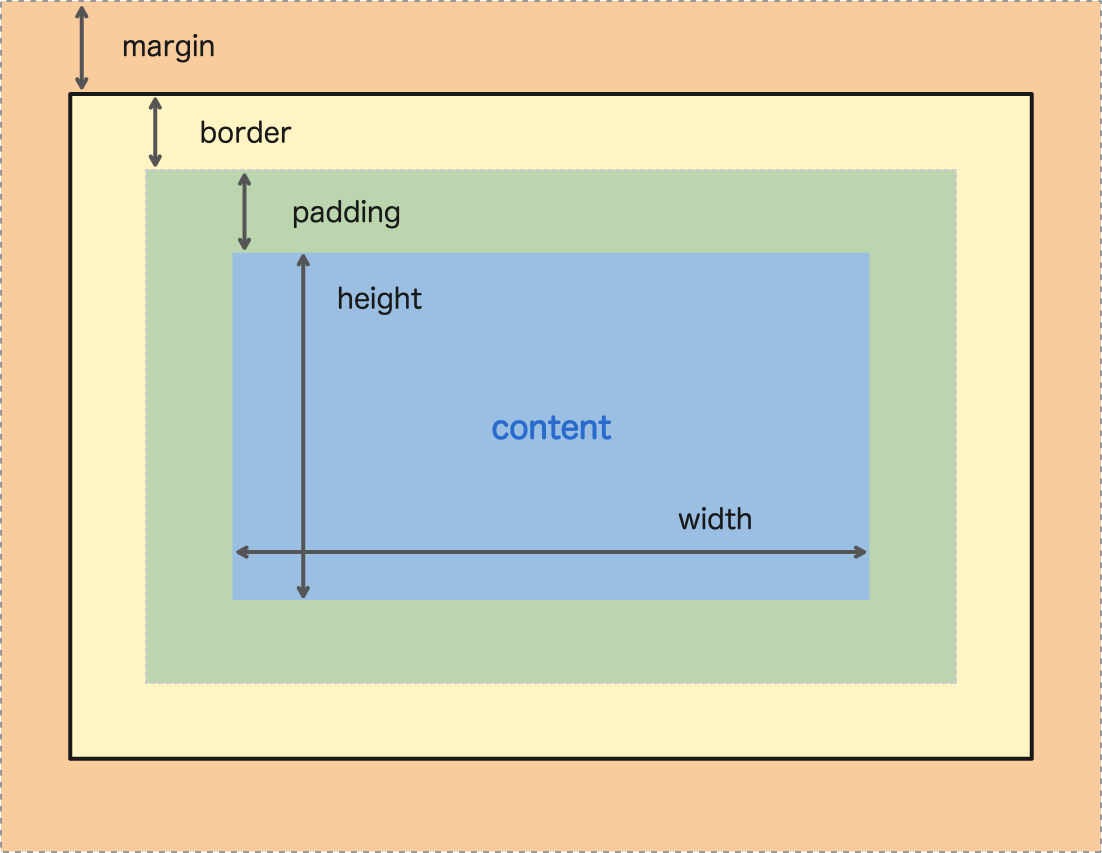
\includegraphics[width=0.6\textwidth]{images/css-box-model.png}
    \caption{The CSS box model}
    \label{fig:cssBoxModel}
\end{figure}

\subsection{Borders}
The CSS \verb|border| property allows you to specify the style, width and colour of an elements border.
\begin{table}[H]
    \centering
    \begin{tabularx}{0.5\textwidth}{X|X}
        Property & Description\\
        \hline
        \verb|dotted| & Dotted border \\
        \verb|dashed| & Dashed border\\
        \verb|solid| & Solid border\\
        \verb|double| & Double border\\
        \verb|groove| & 3D grooved border, effect depends on the \verb|border-color| value\\
        \verb|ridge| & 3D ridged border, effect depends on the \verb|border-color| value\\
        \verb|inset| & 3D inset border, effect depends on the \verb|border-color| value\\
        \verb|outset| & 3D outset border, effect depends on the \verb|border-color| value\\
        \verb|none| & No border\\
        \verb|hidden| & Hidden Border
    \end{tabularx}
    \caption{CSS border options}
    \label{tab:cssBorders}
\end{table}
\subsubsection{Border Width}
The \verb|border-width| property specifies the size of the four borders. The width can be set as a specified size (in \verb|px|, \verb|pt|, \verb|cm|, \verb|em|, etc) or by using on of three pre-defined values \verb|thin|, \verb|medium| or \verb|thick|. Different sides are also able to have different thicknesses. For example, for a solid 5px wide border:
\begin{Verbatim}[breaklines=true, breakanywhere=true]
p.one {
  border-style: solid;
  border-width: 5px;
}
\end{Verbatim}
\subsubsection{Border Colours}
The \verb|border-color| property is used to set the colour of the four borders. If this isn't set then the border inherits the colour of the element.
\subsection{Margins}
The CSS \verb|margin| properties are used to create space around elements, outside any defined borders. With CSS, you have full control over the margins. There are four properties for setting the margin for each side of an element (\verb|top|, \verb|right|, \verb|bottom| and \verb|left|). 
\subsection{Padding}
The CSS \verb|padding| properties are used to generate space around an element's content, inside of any defined borders.
\subsection{Height and Width}
The \verb|height| and \verb|width| properties are used to set the height and width of an element. The \verb|height| and \verb|width| properties do not include padding, borders or margins. It sets the height and width of the area inside the padding, border and margins of the element.
\begin{table}[H]
    \centering
    \begin{tabularx}{0.5\textwidth}{X|X}
        Property & Description\\
        \hline
        \verb|auto| & Default, browser calculates height and width \\
        \verb|length| & Defines the height/ width in px, cm etc\\
        \% Percent Symbol & Defines the height/ width in percent of the containing block\\
        \verb|initial| & Sets the height/ width to its default value\\
        \verb|inherit| & The height/ width will be inherited from its parent value
    \end{tabularx}
    \caption{CSS height and width options}
    \label{tab:cssHeightWidth}
\end{table}
For example
\begin{Verbatim}[breaklines=true, breakanywhere=true]
div {
  height: 100px;
  width: 500px;
  background-color: powderblue;
}
\end{Verbatim}
\subsubsection{Maximum Width}
The \verb|max-width| property is used to set the maximum width of an element. It can be specified in length, values or percent of the containing block. For example
\begin{Verbatim}[breaklines=true, breakanywhere=true]
div {
  max-width: 500px;
  height: 100px;
  background-color: powderblue;
}
\end{Verbatim}

\section{Text}
\subsection{Text Colour}
The \verb|colour| property is used to set the colour of the texti, it is specified by a colour name.
\subsubsection{Text Alignment}
The \verb|text-align| property is used to set the horizontal alignment of a text element. A text element can be left or right justified, centred or justified. For example, to centre align a \verb|<h1>|:
\begin{Verbatim}[breaklines=true, breakanywhere=true]
h1 {
  text-align: center;
}
\end{Verbatim}
When the \verb|text-align| is set to \verb|justify|, each line is stretched so that every line has an equal width therefore the left and right margins are straight.
\subsection{Text Direction}
The \verb|direction| and \verb|unicode-bidi| properties can be used to change the direction of an element. For example
\begin{Verbatim}[breaklines=true, breakanywhere=true]
p {
  direction: rtl;
  unicode-bidi: bidi-override;
}
\end{Verbatim}
\subsection{Vertical Alignment}
The \verb|vertical-align| property sets the vertical alignment of an element.
\subsection{Text Decoration}
The \verb|text-decoration| property is used to set or remove decorations from text. The value \verb|none| is often used to remove underlines from links.
\subsection{Text Transformation}
The \verb|text-transform| property is used to specify uppercase and lowercase letters in a text element. It can be used to turn everything into uppercase or lowercase letters, or capitalise the first letter of each word. 
\subsection{Text Indent}
The \verb|text-indent| property is used to specify the indentation of the first line of text.
\begin{Verbatim}[breaklines=true, breakanywhere=true]
p {
  text-indent: 50px;
}
\end{Verbatim}
\subsection{Letter Spacing}
The \verb|letter-spacing| property is used to specify the space between the characters in a text element.
\subsection{Line Height}
The \verb|line-height| property is used to specify the space between lines.
\subsection{Word Spacing}
The \verb|word-spacing| property is used to specify the space between the words in a text element.
\subsection{White Space}
The \verb|white-space| property is used to specify how white space inside an element is handled.
\subsection{Text Shadow}
The \verb|text-shadow| property adds shadow to text. For example,
\begin{Verbatim}[breaklines=true, breakanywhere=true]
h1 {
  text-shadow: 2px 2px 5px red;
}
\end{Verbatim}

\section{Fonts}
It is important to choose a good font for websites. 
\subsection{Introduction to Fonts}
\begin{itemize}
    \item Serif fonts have small strokes at the edges of each letter. They create a sense of formality and elegance.
    \item Sans-Serif fonts have clean lines (no small strokes). They create a modern and minimalistic look.
    \item Mono space fonts have equal spacing for all letters. They create a mechanical look.
    \item Cursive fonts imitate human handwriting.
    \item Fantasy fonts are decorative or playful fonts.
\end{itemize}

\subsection{Font Families}
The \verb|font-family| property specifies the font of a text. The \verb|font-family| should hold seceral font names as a ``fallback'' system, to ensure maximum compatibility between browser/operating systems. Start with the font you want and end with a generic family (this lets the browser pick a similar font in the family if no other specified fonts are available) the font names should be separated with a comma. If the font name contains more than one word, then it must be in quotation marks. For example
\begin{Verbatim}[breaklines=true, breakanywhere=true]
.p1 {
  font-family: "Times New Roman", Times, serif;
}
\end{Verbatim}
\subsection{Web Safe Fonts}
Web safe fonts are fonts that are universally installed across all browsers and devices. However, there are no 100\% completely safe web fonts. There is always a chance that a font is not found or installed properly. The best web safe fonts for HTML and CSS are shown below.
\begin{itemize}
    \item Arial - sans serif;
    \item Veranda - sans serif;
    \item Helvetica - sans serif;
    \item Tahoma - sans serif;
    \item Trebuchet MS - sans serif;
    \item Times New Roman - serif;
    \item Georgia - serif;
    \item Garamond - serif;
    \item Courier New - mono space;
    \item Brush Script MT - cursive.
\end{itemize}
\subsection{Font Style}
The \verb|font-style| property is mostly used to specify italic text. It has three values: \verb|normal| (text is shown normally); \verb|italic| (text is shown in italics); and \verb|oblique| (text is leaning).
\subsection{Font Weight}
The \verb|font-weight| property specifies the weight of a font. 
\subsection{Font Variant}
The \verb|font-variant| property specifies whether or not a text element should be displayed in a \textsc{small caps} font. In a small-caps font, all lowercase letters are converted to uppercase letters. However the converted uppercase letters appear in a smaller font size than the original uppercase letters in the text.
\subsection{Font Size}
The \verb|font-size| property sets the size of the text. Being able to manage the text size is important in web design. However, you should not use font size adjustments to make paragraphs look like headings or headings look like paragraphs.\\
The \verb|font-size| value can be absolute or relative size. Absolute size sets the text to a specified size, doesn't allow the user to change the text size in browsers (bad for accessibility); it is useful for when the physical size of the output is known. Relative size sets the size of the text to be relative to the surrounding elements and allows a user to change the text size in browsers. For example, to set a font size using pixels
\begin{Verbatim}[breaklines=true, breakanywhere=true]
h1 {
  font-size: 40px;
}
\end{Verbatim}
\subsection{Google Fonts}
If you do not want to use any of the standard fonts in HTML, you can use Google Fonts\footnote{https://fonts.google.com/}. Google Fonts are free to use and have more than 1000 styles. You link them to HTML documents as you would any other style sheet
\begin{Verbatim}[breaklines=true, breakanywhere=true]
<link rel="stylesheet" href="https://fonts.googleapis.com/css?family=Sofia">
\end{Verbatim}

\section{Links}
Links can be styled in different ways. They can be styled with any CSS properties. For example
\begin{Verbatim}[breaklines=true, breakanywhere=true]
a {
  color: hotpink;
}
\end{Verbatim}
In addition, they can be styled differently depending on what state they are in
\begin{table}[H]
    \centering
    \begin{tabularx}{0.5\textwidth}{X|X}
        State & Description\\
        \hline
        \verb|a:link| & unvisited\\
        \verb|a:visited| & visited\\
        \verb|a:hover| & when a mouse hovers over the link\\
        \verb|a:active| & the moment it is 
    \end{tabularx}
    \caption{Different states which a link can be in}
    \label{tab:linkStates}
\end{table}

\chapter{JavaScript}
JavaScript (\textit{JS}) is a widely used programming language that can be used to add interactivity to web pages. It can be used to gather and process data from the user, to create dynamic page elements and to do useful things such as to validate data. The code is interpreted and is mainly used for client-side processing.
\section{Including JavaScript on Webpages}
There are a number of different methods which can be used to include JavaScript in a webpage. 
\subsection{Script Tag}
Small amounts of code can be included in the \verb|<script>| tags. If a time to run (eg, on button press) is not specified then it will run as soon as the webpage is opened. For example, the code below will display an alert box containing ‘hello world’ when the webpage is opened.
\begin{Verbatim}[breaklines=true, breakanywhere=true]
<script>
alert("Hello World!");
</script>
\end{Verbatim}
\subsection{In Separate Files}
This is a more advantageous method of including JS in a webpage as you can use the same JS across multiple pages; HTML documents are less cluttered and easier for the developer to read and the webpage may be faster to load as the linked files can be cached. You include the JS file in the same way that you would include a CSS file as seen below
\begin{Verbatim}[breaklines=true, breakanywhere=true]
<head>
<script src="my_scripts.js"></script>
</head>
\end{Verbatim}

\section{Running JavaScript code}
Using the onclick attribute of HTML elements, it is possible to trigger JS functions. For example, the HTML below
\begin{Verbatim}[breaklines=true, breakanywhere=true]
<button onclick="say_hello()">Press me!</button>
\end{Verbatim}
will run the function below
\begin{Verbatim}[breaklines=true, breakanywhere=true]
function say_hello() {
  alert ("Hello World!"); 
}
\end{Verbatim}
when pressed.

\section{Syntax}
For the A-Level exam, it is only required to know the syntax for the basic programming constructs. Anything further will be introduced in the question. JavaScript lines end with a semi colon \verb|;| .
\subsection{Comments}
These are started with a double slash - \verb|//|
\subsection{Variables}
These are declared with the keyword var then the variable name then the value can be assigned to it.\\
\verb|var age = 4;|
JavaScript is a dynamic typed language, this means all the different types of data types are declared using the keyword \verb|var|.
To change the value in the variable is like in any other programming language\\
\verb|age = 6;|
\subsection{Selection}
JavaScript has if, else and else if statements which can be used to control the flow of the program. An example is seen below.
\begin{Verbatim}[breaklines=true, breakanywhere=true]
if (age >= 18) {
  alert("You are allowed to drink beer");
} else if (age > 16) {
  alert("Nice try. You are not allowed to drink beer.");
} else {
  alert("Here is some lemonade.");
}
\end{Verbatim}
The code doesn’t have to be indented but this can make it more readable whereas the brackets and curly brackets are needed. 
\subsection{Iteration}
\subsubsection{For Loops}
These are written much the same as in other languages. Notice how the count control variable, \verb|i|, is declared within the loop and that \verb|i++| can be used to increment \verb|i|.
\begin{Verbatim}[breaklines=true, breakanywhere=true]
for (var i = 0; i < 5; i++) {
  document.write("Woohoo");
}
\end{Verbatim}
\subsubsection{While Loops}
These are written using the following syntax.
\begin{Verbatim}[breaklines=true, breakanywhere=true]
var i = 0;
while (i < 5) {
  document.write("Woohoo");
  i++;
}
\end{Verbatim}
\subsection{Arrays}
These are declared in the following way
\begin{Verbatim}[breaklines=true, breakanywhere=true]
var colours = ["red", "orange", "yellow"];
\end{Verbatim}
The arrays are based on a zero-based index and do not have fixed size. The length of an array can be obtained by the following
\begin{Verbatim}[breaklines=true, breakanywhere=true]
colours.length
\end{Verbatim}
Notice that the code above does \textit{not} require brackets after the method name.
\subsection{Subroutines}
All subroutines in JavaScript are called functions, they have the option to return a value but don’t have to. 
They are declared with the function keyword and look like the following
\begin{Verbatim}[breaklines=true, breakanywhere=true]
function multiply(num1, num2){
  // multiplies together two numbers
  var total = num1 * num2;
  return total;
}
\end{Verbatim}
Parameters can be passed into functions and if there is a value to be returned it can be done so using the \verb|return| keyword.
\subsection{Output Methods}
There are a number of different ways JavaScript can be outputted to the user.
\subsubsection{Alert Boxes}
This generates a pop-up box within the browser displaying the specified text. Usually, the box will have a single OK button which lets you close the box.
\begin{Verbatim}[breaklines=true, breakanywhere=true]
<script>
alert("Hello!");
</script>
\end{Verbatim}
\subsubsection{Document Write}
This outputs the contents of the brackets at the point at which the \verb|<script>| tag appears in the webpage. This means if you have the \verb|<script>| tag at the top of the page, then the output will be at the top of the page.
\begin{Verbatim}[breaklines=true, breakanywhere=true]
<script>
var result = 2 + 3
document.write(result);
</script>
\end{Verbatim}
You can also include HTML tags to format the output.
\begin{Verbatim}[breaklines=true, breakanywhere=true]
<script>
var result = 2 + 3
document.write("<h1>",result,"</h1>");
</script>
\end{Verbatim}
\subsubsection{Changing The Value Of An Element}
This allows you  to directly change the value inside a HTML element. This works by using the id of the HTML element to set the contents of the tags within the JS code. This can be seen in the following example.
\begin{Verbatim}[breaklines=true, breakanywhere=true]
<h1 id="example">Page heading</h1>
<script>
chosen_element = document.getElementById("example");
chosen_element.innerHTML = "Hello World";
</script>
\end{Verbatim}
\subsection{Input Methods}
HTML forms are widely used across all webpages. The following example shows the HTML for an entire webpage which contains JS in the \verb|<head>| tag and a form in the \verb|<body>| tag. 
\begin{Verbatim}[breaklines=true, breakanywhere=true]
<!DOCTYPE html>
<html>
  <head>
    <script>
        // Define a function which will be called when the button is clicked
        function greeting(){
          // Retrieve the value of the 'firstname' text box
          alert("Hello " + document.getElementById("firstname").value);
          }
    </script>
   </head>
<body>
  <form>
    <p>What is your name?</p> 
    <input type="text" id="firstname">
    <input type="submit" onclick="greeting()">
  </form>
</body>
</html>

\end{Verbatim}
This works by when the button is pressed, the \verb|greeting()| function is run. This displays an alert box with the text entered by the user in it. 


\chapter{References}
\begin{itemize}
    \item W3Schools HTML Tutorial -\\ \href{https://www.w3schools.com/html/default.asp}{https://www.w3schools.com/html/default.asp}
    \item W3Schools CSS Tutorial -\\ \href{https://www.w3schools.com/css/default.asp}{https://www.w3schools.com/css/default.asp}
    \item Isaac Computer Science JavaScript Notes -\\ \href{https://isaaccomputerscience.org/concepts/prog\_gui\_javascript}{https://isaaccomputerscience.org/concepts/prog\_gui\_javascript}
    \item Figure \ref{fig:cssBoxModel} -\\ \href{https://sabe.io/classes/css/css-box-model-padding-border-margin}{https://sabe.io/classes/css/css-box-model-padding-border-margin}
\end{itemize}
\end{document}
% need to add something about javascript woo!

\begin{Verbatim}[breaklines=true, breakanywhere=true]

\end{Verbatim}